Cellular network and power grid operators measure rich timeseries data, such as city-wide mobility and electricity demand patterns. Sharing such data with \textit{external} entities, such as a
taxi fleet operator, can enhance a host of \SC{societal-scale control tasks}, ranging from
taxi routing to battery storage optimization. 
However, how should timeseries owners \textit{represent} their data to limit the scope and volume of information shared across a data boundary, such as a congested wireless network?\footnote{Uber processes petabytes of data per day \cite{Uber} and a mobile operator can process 60 TB of daily cell metrics \cite{SK}. Even a \textit{fraction} of such data is hard to send.}

At a first glance, it might seem sufficient to simply share generic demand forecasts with any downstream controller.
Each controller, however, often has a unique cost function and context-specific sensitivity to prediction errors.
%, which are often \textit{unknown} to the timeseries generator. 
For example, cell demand forecasts should emphasize accurate peak-hour forecasts for taxi fleet routing. The same underlying cellular data should instead emphasize fine-grained throughput forecasts when a video streaming controller starts a download. 
Despite the benefits of customizing forecasts for control, today's forecasts are mostly \textit{task-agnostic} and simply optimize for mean or median prediction error. As such, they often waste valuable network bandwidth to transmit temporal features that are unnecessary for a downstream controller. Even worse, they might not minimize errors when they matter most, such as peak-hour variability.
%Even worse, they often don't minimize error when it matters most, such as peak-hour variability.

% check
% \begin{figure}[t]
% \vskip 0.2in
% \begin{center}
% \centerline{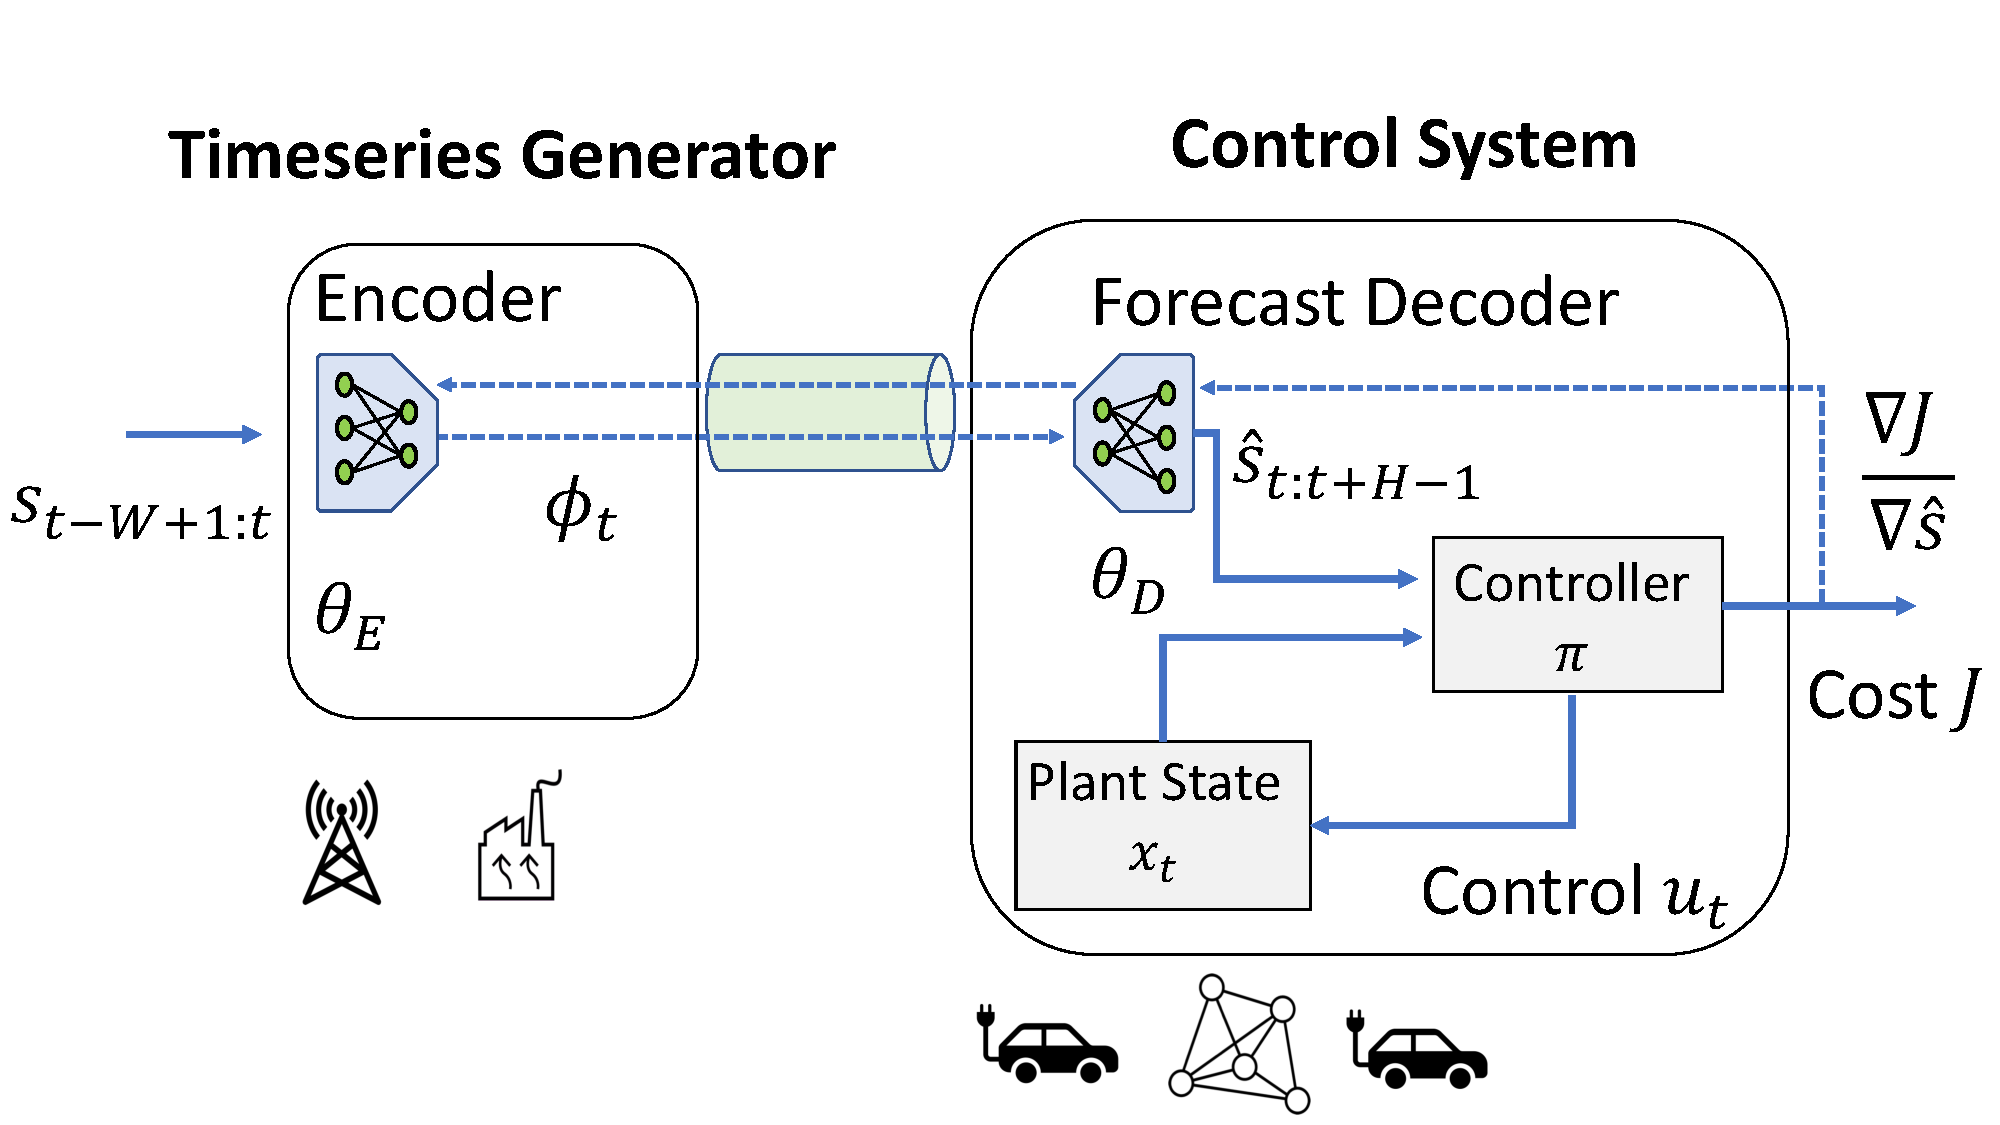
\includegraphics[width=0.6\columnwidth]{figures/final_model_nabla_2.pdf}}
% \caption{\textbf{Data sharing for cooperative control:} An owner of timeseries data $s_t$, such as a mobile operator, needs to transmit a compressed representation $\phi_t$ to a downstream controller with internal state $x_t$. The \textit{learned} forecast emphasizes task-relevant temporal features to minimize end-to-end controller cost $J$.} 
% \label{fig_problem}
% \end{center}
% \vskip -0.4in
% \end{figure}

\begin{wrapfigure}{R}{0.5\columnwidth}
\centering
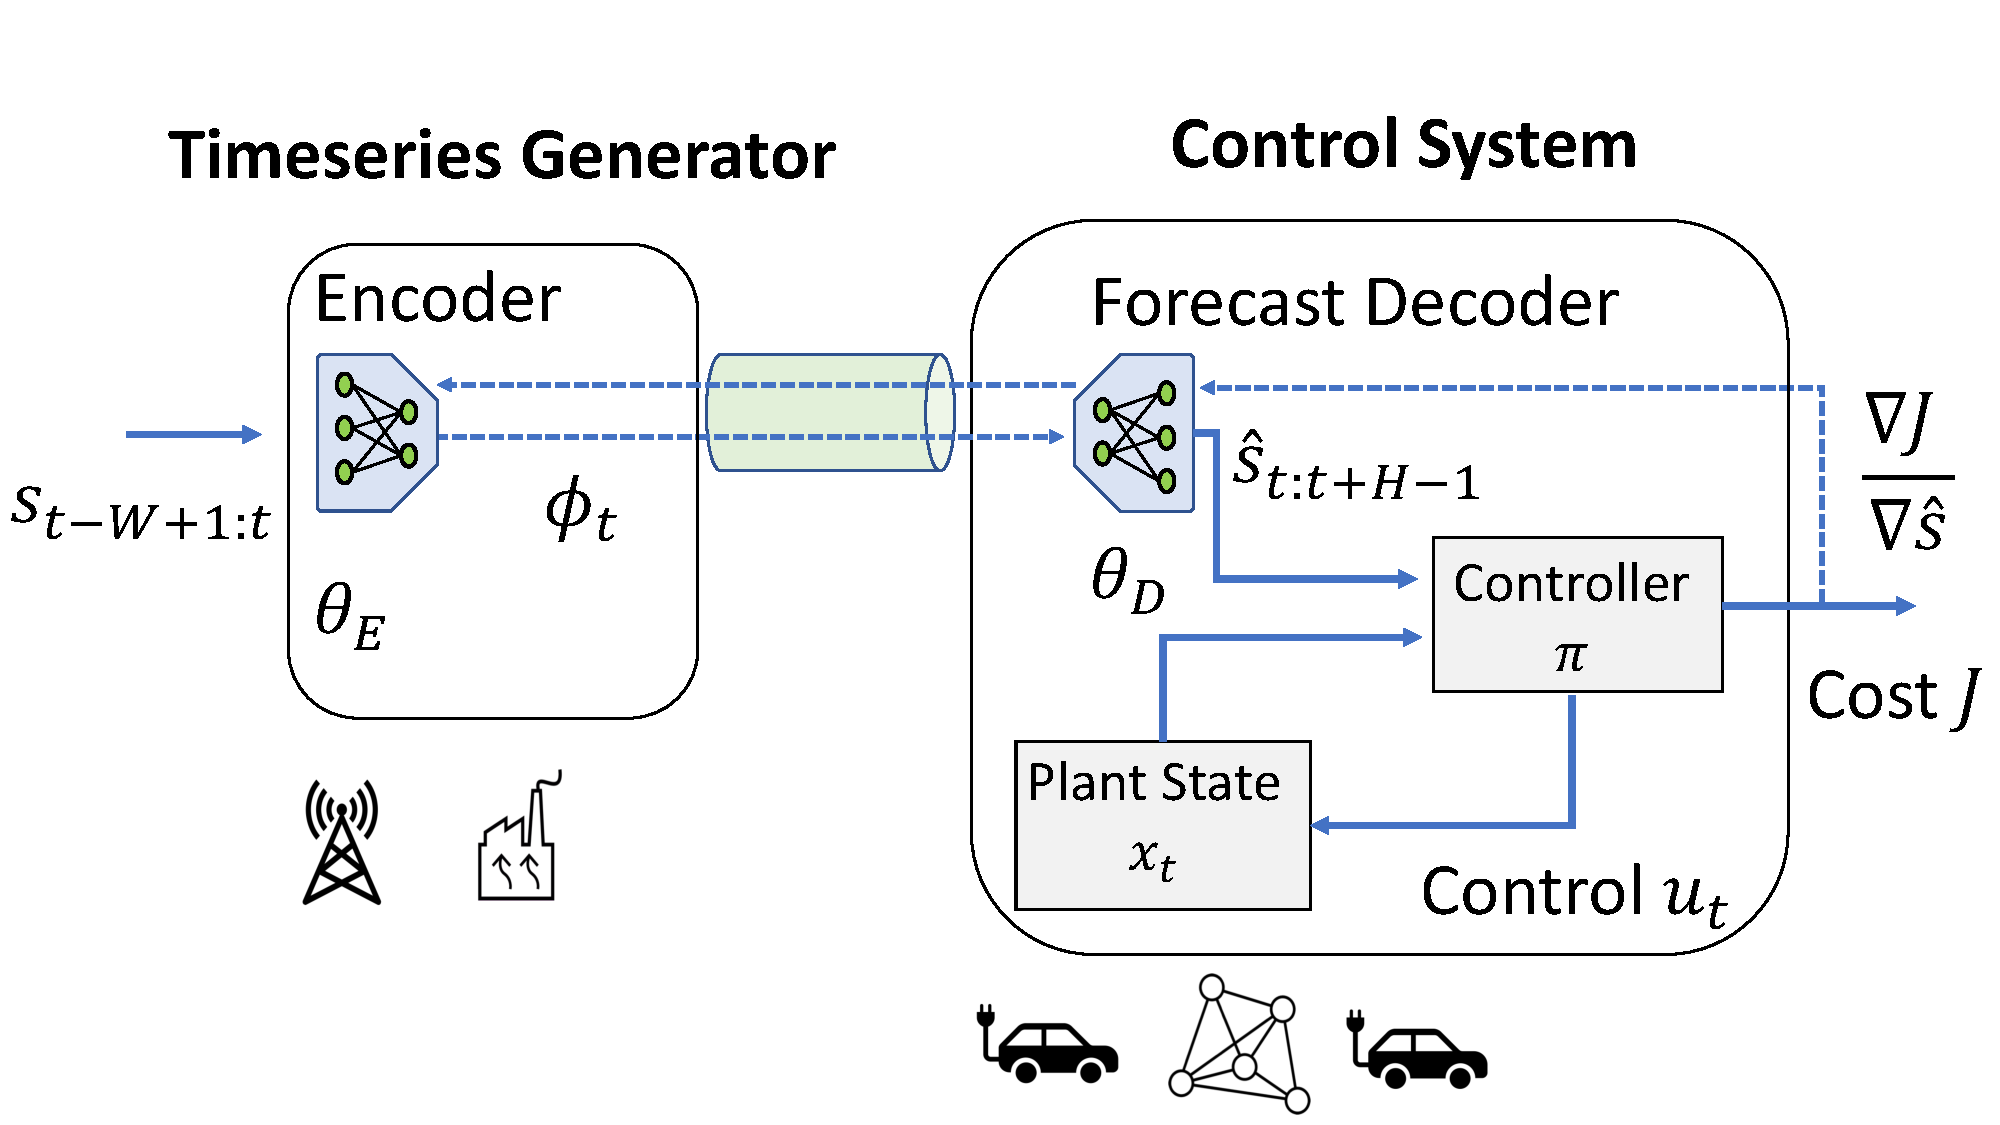
\includegraphics[width=0.5\columnwidth]{figures/final_model_nabla_2.pdf}
\caption{\textbf{Data sharing for cooperative control:} An owner of timeseries data $s_t$, such as a mobile operator, needs to transmit a compressed representation $\phi_t$ to a downstream controller with internal state $x_t$. The \textit{learned} forecast emphasizes task-relevant temporal features to minimize end-to-end controller cost $J$.}
\label{fig_problem}
% \vskip -0.5em
\end{wrapfigure}


Given the limitations of today's task-agnostic forecasts, this paper contributes a novel problem formulation for learning \textit{task-driven} forecasts for networked control. 
In our general problem (Fig. \ref{fig_problem}), an operator measures timeseries $s_t$, such as electricity or cell demand, and 
transmits compressed representation $\phi_t$, which is decoded to $\hat{s}_t$ at the controller. Rather than simply minimize the prediction error for $\hat{s}_t$, we instead learn a representation that minimizes a modular controller $\pi$'s ultimate cost $J$.
Our key technical insight is to compute a controller's sensitivity to prediction errors, which in turn guides how we \textit{co-design} and learn a concise forecast representation that is tailored to control. 
As such, our scheme jointly integrates data-driven forecasting, compression, and model-based control. 
%As such, we can jointly integrate data-driven forecasting with data compression and model-based control. 
%As such, we can blend data-driven forecasting with model-based control. 
%that is co-designed with a model-based controller.

%As such, we can interface a data-driven forecaster that is co-designed with the task objective of a model-based controller.
%by separating but \textit{co-designing} forecasting and control, we can blend model-based control with data-driven forecasters.
%Crucially, we can blend model-based control with data-driven forecasting by propagating a classical controller's sensitivity to forecasts to a modular forecaster's learned parameters.
%Morever, our approach allows us to blend neural network forecasters with model-based control by compart
%Our key technical insight is to \textit{co-design} and learn a compressed forecast representation tailored to a model-based controller, which allows us to blend data-driven forecasting and classical control. 
%techniques. 
%This insight allows us to learn representations that are $80\%$ smaller than those generated by standard autoencoders, even for real IoT sensor data we captured on embedded devices as well as standard benchmark datasets.
%Our key technical insight is to propagate a controller's sensitivity to prediction errors to guide learning of a modular forecasting model. As such, we can \textit{co-design} and learn a concise forecast representation that is tailored to a model-based controller, allowing us to seamlessly blend data-driven forecasting and classical control.
%Our key technical insight is to propagate a controller's sensitivity to prediction errors back to the modular forecasting model that generates such predictions. As such, we can \textit{co-design} and learn a concise forecast representation that is tailored to a model-based controller, allowing us to seamlessly blend data-driven forecasting and classical control.
%which in turn guides how we \textit{co-design} and learn a concise forecast representation tailored to control. As such, we can seamlessly blend classical model-based control with neural network forecasting models.

\tu{Related work:} 
Our work is broadly related to information-theoretic compression for control as well as task-driven representation learning. The closest work to ours is \cite{donti2017task}, where task-driven forecasts are learned for one-step stochastic optimization problems. In stark contrast, we address \textit{compression} of timeseries forecasts and focus on networked, multi-step control problems. Our work is also inspired by Shannon's rate-distortion theory \cite{berger2003rate}, which describes how to encode and transmit signals with a minimal bit-rate to minimize reconstruction error.
%\SC{In contrast, we observe that if we optimize for control cost, as opposed to simply reconstruction error, we can achieve
%significantly better compression gains by encoding only task-relevant features}.
%a forecast should only encode task-relevant features necessary to minimize control cost, which enables significant compression gains compared to optimizing for reconstruction error. 
In contrast, we work with real numbers rather than bits and focus on reducing the dimension of data while keeping task-specific control cost low.

%We observe that a forecast should only encode task-relevant features necessary to minimize control cost, which enables significant compression gains compared to optimizing for reconstruction error. Our distortion measure is task specific.

Prior work has addressed rate-distortion tradeoffs for networked LQR control problems \cite{kostina2019rate,tatikonda2004stochastic,schenato2007foundations}. However, these works focus on ensuring closed-loop stability for a remote controller and a physically-separated plant, \SC{such as in tele-operation}. Our problem is fundamentally different, since we address how \textit{external} timeseries forecasts can enhance a controller's \textit{local} decisions using full knowledge of its own internal state. 
\SC{While the term \textit{co-design} appears in select work on networked LQR, it refers to a drastically different setting where a communication scheduler and tele-operated controller must be jointly designed \cite{yun2011optimal,zhang2006communication,branicky2002scheduling,peng2013event}}. 
\JC{
Moreover, event-triggered control/learning \cite{heemels2012introduction,miskowicz2018event,schluter2020event,beuchert2020overcoming} emphases temporal sparsity of communications, while in our setting the MPC controller consistently requires a forecast of timeseries.
}
Finally, our work differs from deep neural network (DNN) compression schemes for video inference \cite{blau2019rethinking,DBLP:conf/rss/NakanoyaCADKP21} since we focus on control.
%that optimize for either human or machine perception tasks \cite{blau2019rethinking,nakanoya2020task} since we focus on multi-step control.


\JC{
More discussions will follow in Sec. \ref{sec:problem_statement} after the technical problem is introduced in detail.
}

\tu{Contributions:}
In light of prior work, our contributions are three-fold. First, we introduce a novel problem for learning compressed timeseries representations that are tailored to control. 
%Second, we illustrate how to use a controller's sensitivity to prediction errors to guide data-driven learning of concise, task-relevant forecasts.
%Second, we show how to compute a 
%controller's sensitivity to prediction errors, which guides learning of concise forecast representations as well as analytical compression results for linear control.
Second, to gain insights into our problem, we contribute analytic compression results for LQR control. These insights serve as a foundation for our general algorithm that computes the sensitivity of a model predictive controller (MPC) to prediction errors, which guides learning of concise forecast representations.
%Second, we contribute analytic compression results for LQR control, which serve as foundations for our model predictive control (MPC) experiments. Third, we illustrate the generality and efficacy of our approach using DNN forecasts for real cell, IoT, and electricity grid data. 
Third, we learn representations that improve control performance by $>25\%$ and are $80\%$ smaller than those generated by standard autoencoders, even for real IoT sensor data we captured on embedded devices as well as benchmark electricity and cell datasets.
%In particular, we collect timeseries from an embedded IoT sensor for our experiments.

\tu{Organization:} 
%This paper is organized as follows. 
In Sec. \ref{sec:problem_statement}, we formalize a general problem of compression for networked control and provide analytical results for LQR. Then, in Sec. \ref{sec:algorithm}, we contribute an algorithm for task-driven data compression for general MPC problems. We demonstrate strong empirical performance of our algorithm for cell, energy, and IoT applications in Sec. \ref{sec:scenarios} - \ref{sec:evaluation} and conclude in Sec. \ref{sec:conclusion}.

%We demonstrate strong empirical performance of our compression scheme for cellular traffic scheduling, energy forecasting, and control from IoT sensors in Sec. \ref{sec:scenarios} - \ref{sec:evaluation}. Finally, we conclude in Sec. \ref{sec:conclusion}.
